%%%%%%%%%%%%%%%%%%%%%%%%%%%%%%%%%%%%%%%%%%%
%
% From a template maintained at https://github.com/jamesrobertlloyd/cbl-tikz-poster
%
% Code near the top should be fairly standard and not need to be changed
%  - except for the document class
% Code lower down is more likely to be customised
%
%%%%%%%%%%%%%%%%%%%%%%%%%%%%%%%%%%%%%%%%%%%


\documentclass[landscape,a1,final,a4resizeable]{include/a0poster}

%%% Packages %%%%%%%%%%%%%%%%%%%%%%%%%%%%%%%%%%%%%%%%%%%%%%%%%%%%%%%%%


\usepackage{multicol}
\setlength{\columnseprule}{0pt}
\def\columnseprulecolor{\color{white}}
% \usepackage[srgb]{xcolor}
\usepackage{morefloats}
\usepackage[pdftex]{graphicx}
\usepackage{rotating}
\usepackage{amsmath, amsthm, amssymb, bm}
\usepackage{array}
\usepackage{booktabs}
%\usepackage{shortcuts}
\usepackage{multirow}
\usepackage{hyperref}
\usepackage[margin=1.5cm]{geometry}
\usepackage[pan gram]{blindtext}
\usepackage{setspace}
\usepackage[dvipsnames]{xcolor}
\usepackage{mwhmacros}
\usepackage{include/picins}
\usepackage{tikz}
\usetikzlibrary{shapes.geometric,arrows,chains,matrix,positioning,scopes,calc}
\tikzstyle{mybox} = [draw=black, rectangle]
\usepackage{dsfont}
%%%%%%%%%%%%%%%%%%%%%%%%%%%%%%%%%%%%%%%%%%%
%
% myfig
%
% \myfig - replacement for \figure
% necessary, since in multicol-environment 
% \figure won't work        
%                 
%%%%%%%%%%%%%%%%%%%%%%%%%%%%%%%%%%%%%%%%%%%

\newcommand{\myfig}[3][0]{
\begin{center}
  \vspace{1.5cm}
  \includegraphics[width=#3\hsize,angle=#1]{#2}
  \nobreak\medskip
\end{center}}

%%%%%%%%%%%%%%%%%%%%%%%%%%%%%%%%%%%%%%%%%%%
%
% mycaption                
%
% \mycaption - replacement for \caption
% necessary, since in multicol-environment \figure and
% therefore \caption won't work
%
%%%%%%%%%%%%%%%%%%%%%%%%%%%%%%%%%%%%%%%%%%%

%\newcounter{figure}
\setcounter{figure}{1}
\newcommand{\mycaption}[1]{
  \vspace{0.5cm}
  \begin{quote}
    {{\sc Figure} \arabic{figure}: #1}
  \end{quote}
  \vspace{1cm}
  \stepcounter{figure}
}

%%%%%%%%%%%%%%%%%%%%%%%%%%%%%%%%%%%%%%%%%%%
%
% Some standard colours
%
%%%%%%%%%%%%%%%%%%%%%%%%%%%%%%%%%%%%%%%%%%%

\definecolor{camLightBlue}{rgb}{.416,.678,.894}
\definecolor{camdarkblue}{rgb}{0, 0.203, 0.402}
\definecolor{camred}{rgb}{1, 0.203, 0}
\definecolor{camyellow}{rgb}{1, 0.8, 0}
\definecolor{lightblue}{rgb}{0, 0, 0.80}
\definecolor{white}{rgb}{1, 1, 1}
\definecolor{whiteblue}{rgb}{0.80, 0.80, 1}

%%%%%%%%%%%%%%%%%%%%%%%%%%%%%%%%%%%%%%%%%%%
%
% Some look and feel definitions
%
%%%%%%%%%%%%%%%%%%%%%%%%%%%%%%%%%%%%%%%%%%%

\setlength{\columnsep}{0.03\textwidth}
\setlength{\columnseprule}{0.0018\textwidth}
\setlength{\parindent}{0.0cm}

%%%%%%%%%%%%%%%%%%%%%%%%%%%%%%%%%%%%%%%%%%%
%
% \mysection - replacement for \section*
% 
% Puts a pretty box around some text
% TODO - any other thoughts for what this box should look like
%
%%%%%%%%%%%%%%%%%%%%%%%%%%%%%%%%%%%%%%%%%%%

\tikzstyle{mysection} = [rectangle, 
			draw=none, 
			shade, 
			outer color=camLightBlue!100,
			inner color=camLightBlue!100,
			text width=0.965\columnwidth,
			text centered,
			rounded corners=20pt,
			minimum height=0.09\columnwidth]

\newcommand{\mysection}[1]
{
\begin{center}
  \begin{tikzpicture}
    \node[mysection] {\sffamily\bfseries\Large\textcolor{white}{#1}};
  \end{tikzpicture}
\end{center}
}

%%%%%%%%%%%%%%%%%%%%%%%%%%%%%%%%%%%%%%%%%%%
%
% Set the font
%
% TODO - Not sure what a canonical choice is - feel free to modify
%
%%%%%%%%%%%%%%%%%%%%%%%%%%%%%%%%%%%%%%%%%%%

\renewcommand{\familydefault}{cmss}
\sffamily

%%%%%%%%%%%%%%%%%%%%%%%%%%%%%%%%%%%%%%%%%%%%%%%%%%%%
%%%               Background                     %%%
%%%%%%%%%%%%%%%%%%%%%%%%%%%%%%%%%%%%%%%%%%%%%%%%%%%%

\newcommand{\background}[3]{
  \definecolor{cgradbegin}{#1}
  \definecolor{cgradend}{#2}
 \psframe[fillstyle=gradient,gradend=cgradend,
 gradbegin=cgradbegin,gradmidpoint=#3](0.,0.)(1.\textwidth,-1.\textheight)
}




%%%%%%%%%%%%%%%%%%%%%%%%%%%%%%%%%%%%%%%%%%%%%%%%%%%%
%%%                pcolumn                       %%%
%%%%%%%%%%%%%%%%%%%%%%%%%%%%%%%%%%%%%%%%%%%%%%%%%%%%

\newenvironment{pcolumn}[1]{
  \begin{minipage}{#1\textwidth}
  \begin{center}
}{
  \end{center}
  \end{minipage}
}



%%%%%%%%%%%%%%%%%%%%%%%%%%%%%%%%%%%%%%%%%%%%%%%%%%%%
%%%                pbox                          %%%
%%%%%%%%%%%%%%%%%%%%%%%%%%%%%%%%%%%%%%%%%%%%%%%%%%%%

\definecolor{lcolor}{rgb}{0, 0, 0.80}
\definecolor{gcolor1}{rgb}{1, 1, 1}
\definecolor{gcolor2}{rgb}{.80, .80, 1}

  \def\fc{fillcolor}
  \def\getfc #1=#2\par{\def\ffc{#1} \ifx\ffc\fc #2\fi} 
  \def\getfillcolor #1,#2\par{\getfc #1\par \getfc #2\par}

  \newcommand{\psshadowbox}[2]{%[2][magenta]{
     \fbox{Input arg: #1}
     \fbox{#1} 
     \fbox {\getfillcolor #1\par}
     \def\col{\getfillcolor #1\par}
 
     \let\coll=\col
      \coll
     \colorbox{\col}{#2}
      \mbox
     \coloredshadowbox{black}{\coll}{#2}
  }

\newcommand{\pbox}[4]{
%\psshadowbox[#3]{
%\fbox{
\mbox{
\begin{minipage}[t][#2][t]{#1}
#4
\end{minipage}
}%}
}

%%%%%%%%%%%%%%%%%%%%%%%%%%%%%%%%%%%%%%%%%%%
%
% Poster environment
%
% Centres everything and can be used to define the width of the content
%
%%%%%%%%%%%%%%%%%%%%%%%%%%%%%%%%%%%%%%%%%%%

\newenvironment{poster}{
  \begin{center}
  \begin{minipage}[c]{\textwidth}
}{
  \end{minipage}
  \end{center}
}

\def\newarrow{\mbox{\begin{tikzpicture}
             \useasboundingbox{(-3pt,-4.5pt) rectangle (19pt,1pt)};
             \draw[->] (0,-0.07)--(17pt,-0.07);\end{tikzpicture}}}


% \ProvidesPackage{preamble}

\usepackage{url}
\usepackage{array}
\usepackage{amsmath,amssymb,amsfonts,textcomp}
\usepackage{booktabs}
\usepackage{relsize}
\usepackage{nicefrac}
\usepackage{graphicx}
\usepackage{rotating}
\usepackage{nth}
\usepackage{acronym}
\usepackage{bm}

\newcommand{\binarysum}{\sum_{\bf{x} \in \{0,1\}^D}}
\newcommand{\expect}{\mathbb{E}}
\newcommand{\expectargs}[2]{\mathbb{E}_{#1} \left[ {#2} \right]}
\newcommand{\var}{\mathbb{V}}
\newcommand{\varianceargs}[2]{\mathbb{V}_{#1} \left[ {#2} \right]}
\newcommand{\variance}{\mathbb{V}}
\newcommand{\cov}{\operatorname{cov}}
\newcommand{\Cov}{\operatorname{Cov}}
\newcommand{\covarianceargs}[2]{\Cov_{#1} \left[ {#2} \right]}
\newcommand{\colvec}[2]{\left[ \begin{array}{c} {#1} \\ {#2} \end{array} \right]}
\newcommand{\tbtmat}[4]{\left[ \begin{array}{cc} {#1} & {#2} \\ {#3} & {#4} \end{array} \right]}

%\newcommand{\covskinny}[2]{\var\!\left(#1\middle\vert#2\right)} 

\newcommand{\acro}[1]{\textsc{#1}}
%\newcommand{\vect}[1]{\boldsymbol{#1}}
\newcommand{\vect}[1]{{\bf{#1}}}
\newcommand{\mat}[1]{\mathbf{#1}}
\newcommand{\pderiv}[2]{\frac{\partial #1}{\partial #2}}
\newcommand{\npderiv}[2]{\nicefrac{\partial #1}{\partial #2}}

\newcommand{\pha}{^{\phantom{:}}}

\newcommand{\argmin}{\operatornamewithlimits{argmin}}
\newcommand{\argmax}{\operatornamewithlimits{argmax}}

% The following designed for probabilities with long arguments

\newcommand{\Prob}[2]{P\!\left(\,#1\;\middle\vert\;#2\,\right)}
\newcommand{\ProbF}[3]{P\!\left(\,#1\!=\!#2\;\middle\vert\;#3\,\right)}
\newcommand{\p}[2]{p\!\left(#1\middle\vert#2\right)}
\newcommand{\po}[1]{p\!\left(#1\right)}
\newcommand{\pF}[3]{p\!\left(\,#1\!=\!#2\;\middle\vert\;#3\,\right)} 
\newcommand{\mean}[2]{{m}\!\left(#1\middle\vert#2\right)}
%\newcommand{\novmean}[2]{{m}\!\left(#1\middle\vert#2\right)}
%\newcommand{\novcov}[2]{\var\!\left(#1\middle\vert#2\right)}
%\newcommand{\cov}[2]{\var\!\left(#1\middle\vert#2\right)} 
%\newcommand{\pskinny}[2]{p\!\left(#1\;\middle\vert\;#2\right)}
%\newcommand{\meanskinny}[2]{{m}\!\left(#1\middle\vert#2\right)}
%\newcommand{\covskinny}[2]{\var\!\left(#1\middle\vert#2\right)} 

\newcommand{\vI}{\mat{I}}
\newcommand{\vX}{\mat{X}}
\newcommand{\vY}{\mat{Y}}
\newcommand{\vZ}{\mat{Z}}
\newcommand{\vK}{\mat{K}}
\newcommand{\vs}{\vect{s}}
\newcommand{\va}{\vect{a}}
\newcommand{\vA}{\vect{A}}
\newcommand{\vb}{\vect{b}}
\newcommand{\vB}{\mat{B}}
\newcommand{\vR}{\mat{R}}
\newcommand{\vS}{\mat{S}}
\newcommand{\vu}{\vect{u}}
\newcommand{\vk}{\vect{k}}
\newcommand{\vc}{\vect{c}}
\newcommand{\vC}{\mat{C}}
\newcommand{\vw}{\vect{w}}
\newcommand{\vx}{\vect{x}}
\newcommand{\vy}{\vect{y}}
\newcommand{\vz}{\vect{z}}
\newcommand{\vmu}{\vect{\mu}}
\newcommand{\vpi}{\vect{\pi}}
\newcommand{\vphi}{\vect{\phi}}
\newcommand{\vSigma}{\mat{\Sigma}}
\newcommand{\vtheta}{\vect{\theta}}
\newcommand{\vl}{\vect{l}}
\newcommand{\vq}{\vect{q}}
\newcommand{\vf}{\vect{f}}
\newcommand{\vg}{\vect{g}}
\newcommand{\vell}{\vect{\ell}}
\newcommand{\ve}{\vect{\epsilon}}
\newcommand{\vzero}{\vect{0}}
\newcommand{\vone}{\vect{1}}

\newcommand{\He}{\mathcal{H}}
\newcommand{\normx}[2]{\left\|#1\right\|_{#2}}
\newcommand{\Hnorm}[1]{\normx{#1}{\He}}
\newcommand{\mmd}{{\rm MMD}}


\newcommand{\mf}{\bar{\vf}}

\newcommand{\st}{_\star}

\newcommand{\inv}{^{{\mathsmaller{-1}}}}
\newcommand{\tohalf}{^{{\mathsmaller{\nicefrac{1}{2}}}}}

\newcommand{\N}[3]{\mathcal{N}\!\left(#1|#2,#3\right)}
\newcommand{\bN}[3]{\mathcal{N}\big(#1|#2,#3\big)}
\newcommand{\boldN}[3]{\text{\textbf{\mathcal{N}}}\big(#1;#2,#3\big)}
\newcommand{\ones}[1]{\mat{1}_{#1}}
\newcommand{\eye}[1]{\mat{E}_{#1}}
\newcommand{\tra}{^\ensuremath{\mathsf{T}}}
\newcommand{\trace}{\operatorname{tr}}
\newcommand{\deq}{:=}
\newcommand{\degree}{^\circ}

\DeclareMathOperator{\chol}{chol}
\DeclareMathOperator{\diag}{diag}

\newcommand{\gp}{{\acro{gp}}}
\newcommand{\bmc}{{\acro{bmc}}}
\newcommand{\bq}{{\acro{bq}}}
\newcommand{\sbq}{{\acro{sbq}}}

\newenvironment{narrow}[2]{%
  \begin{list}{}{%
  \setlength{\topsep}{0pt}%
  \setlength{\leftmargin}{#1}%
  \setlength{\rightmargin}{#2}%
  \setlength{\listparindent}{\parindent}%
  \setlength{\itemindent}{\parindent}%
  \setlength{\parsep}{\parskip}}%
\item[]}{\end{list}}

\newtheorem{prop}{Proposition}
\newtheorem{cor}{Corollary}
\newtheorem{lem}{Lemma}


\def\ie{i.e.\ }
\def\eg{e.g.\ }
\def\iid{i.i.d.\ }
\def\simiid{\sim_{\mbox{\tiny iid}}}
\def\eqdist{\stackrel{\mbox{\tiny d}}{=}}

\def\Reals{\mathbb{R}}

\def\Uniform{\mbox{\rm Uniform}}
\def\Bernoulli{\mbox{\rm Bernoulli}}
\def\GP{\mathcal{GP}}

\def\inputVar{x}
\def\InputVar{X}
\def\InputSpace{\mathcal{X}}
\def\outputVar{y}
\def\OutputSpace{\mathcal{Y}}
\def\function{f}
\def\kernel{k}
\def\KernelMatrix{K}
\def\SumKernel{\sum}
\def\ProductKernel{\prod}
\def\expression{e}

\def\SE{\acro{SE}}
\def\Per{\acro{Per}}
\def\RQ{\acro{RQ}}
\def\Lin{\acro{Lin}}

\def\subexpr{{\cal S}}
\def\baseker{{\cal B}}
\def\numWinners{k}

\newcommand{\kSE}{{\acro{SE}}}
\newcommand{\kC}{{\acro{C}}}
\newcommand{\kPer}{{\acro{Per}}}
\newcommand{\kLin}{{\acro{Lin}}}
\newcommand{\kWN}{{\acro{WN}}}
\newcommand{\kCP}{{\acro{CP}}}
\newcommand{\kCW}{{\acro{CW}}}
\newcommand{\kRQ}{{\acro{RQ}}}


%%% Commands %%%%%%%%%%%%%%%%%%%%%%%%%%%%%%%%%%%%%%%%%%%%%%%%%%%%%%%%%
\newcommand{\X}{\B X}

\newcommand{\elbo}{\mathcal{L}}
\newcommand{\entropy}{\mathbb{H}}
\newcommand{\kl}{\mathbb{K}\mathbb{L}}
\newcommand{\eqnn}[1]{\begin{align}{#1}\end{align}}
\newcommand{\eqn}[1]{\begin{align*}{#1}\end{align*}} 
\newcommand{\D}{\mathcal{D}}
\newcommand{\bb}[1]{\ensuremath{ \left( {#1} \right)}}
\newcommand{\BB}[1]{\ensuremath{\left[ {#1} \right]}} 
\newcommand{\half}{\frac{1}{2}}
\newcommand{\B}[1]{\ensuremath{  \mathbf{#1} } }
\newcommand{\pbnn}{p_{\text{\tiny BNN}}}
\newcommand{\pgp}{p_{\text{\tiny GP}}}
\newcommand{\amin}[1]{\underset{#1}{\text{argmin }}}
\newcommand{\myItem}{\item[\color{camLightBlue}$\bullet$]}
\newcommand{\col}[1]{{\color{camLightBlue}\textbf{#1}}}%{\fbox{#1}}
% \newcommand{\myBox}[1]{\fbox{#1}}%{#1}%

%%% Color Definitions %%%%%%%%%%%%%%%%%%%%%%%%%%%%%%%%%%%%%%%%%%%%%%%%%%%%%%%%%
\definecolor{camBlue}{rgb}{.629,.757,.678}
\definecolor{camLightBlue}{rgb}{.416,.678,.894}
\definecolor{camDarkBlue}{rgb}{.208,.339,.447}
\definecolor{darkgreen}{rgb}{0,0.8,0}
\definecolor{darkblue}{rgb}{0,0.08,0.45}
\definecolor{blue}{rgb}{0,0,1}
%\definecolor{bordercol}{RGB}{40,40,40}
%\definecolor{bordercol}{RGB}{150,150,150}
\definecolor{bordercol}{RGB}{0,0,0}
%\definecolor{headercol1}{RGB}{186,215,230}
\definecolor{headercol1}{RGB}{200,200,200}
%\definecolor{headercol2}{RGB}{80,80,80}
\definecolor{headercol2}{RGB}{255,255,255}
%\definecolor{headerfontcol}{RGB}{0,0,255}
\definecolor{headerfontcol}{RGB}{0,0,0}
%\definecolor{boxcolor}{RGB}{186,215,230}
\definecolor{boxcolor}{RGB}{255,255,255}


%%% Eye Cacther %%%%%%%%%%%%%%%%%%%%%%%%%%%%%%%%%%%%%%%%%%%%%%%%%%%%%%%%%%%%%%%

\begin{document}
\begin{minipage}[t][0pt]{\linewidth}
\hspace{-8cm} 
%Align with edge of page, not margin
\vspace{-1.5cm}

\begin{tikzpicture}[overlay]
    \draw [fill=camLightBlue,draw=none] (0, 5) rectangle (100,-6.9);
    \draw [fill=camLightBlue,draw=none] (0, -56.7) rectangle (100,-100);
\end{tikzpicture}

{
\hspace{-0cm}%
\parbox{.08\textwidth}{\hspace{-2cm} 
  % \vspace{-.5cm}
  
\includegraphics[height=8cm]{badges/Utoronto_badge} \hspace{-4cm}%
} 
\parbox{.09\textwidth}{\hspace{-1cm}
  \vspace{-.5cm}\mbox{\includegraphics[height=6cm]{badges/cambridge_badge} \hspace{1cm}}
  }
\hspace{-2cm}
\parbox{.75\textwidth}{
  \vspace{0.5cm}%
  \begin{center}\color{white}
   \Huge \textbf{Mapping Gaussian Processes to Bayesian Neural Networks}\vspace{3mm}\\
    \huge Daniel Flam-Shepherd$^{\,1}$, James Requeima$^{\,2\,3}$, David Duvenaud$^{\,1}$\\
    \color{white}\large 
    $1$ University of Toronto, $2$ University of Cambridge, $3$ Invenia Labs
    \end{center}
  }%
\hspace{1cm}
\parbox{.05\textwidth}{  
  \begin{flushright}\vspace{0.5cm}
\includegraphics[height=6cm]{badges/inv_labs}\hfill% 
  \end{flushright}}
}%


%%%  Main Body %%%%%%%%%%%%%%%%%%%%%%%%%%%%%%%%%%%%%%%%%%%%%%%%%%%%%%%%%%%%%%%

\begin{poster}%
% Potentially add some space at the top of the poster
\vspace{0\baselineskip}%
\vspace*{0.7cm}%
\large%
\noindent%

\begin{multicols}{3}

%%% First Column %%%%%%%%%%%%%%%%%%%%%%%%%%%%%%%%%%%%%%%%%%%%%%%%%%%%%%%%%%%%%%%

\begin{minipage}[t][47.5cm][t]{.32\textwidth}



\mysection{Priors in Function Space are Interpretable}{

%\vspace{-1cm}
\begin{itemize}
  \item \col{\bf Baysian Neural Network Priors} are specified in parameter space. The implications of these priors in function space are hard to interpret.
  \item How to we incorporate prior knowledge about function properties in our prior?
  \item \col{Gaussian Processes} can elegantly  incorporate prior beliefs about functions through the mean and covariance functions.
\end{itemize}
\vspace{1cm}
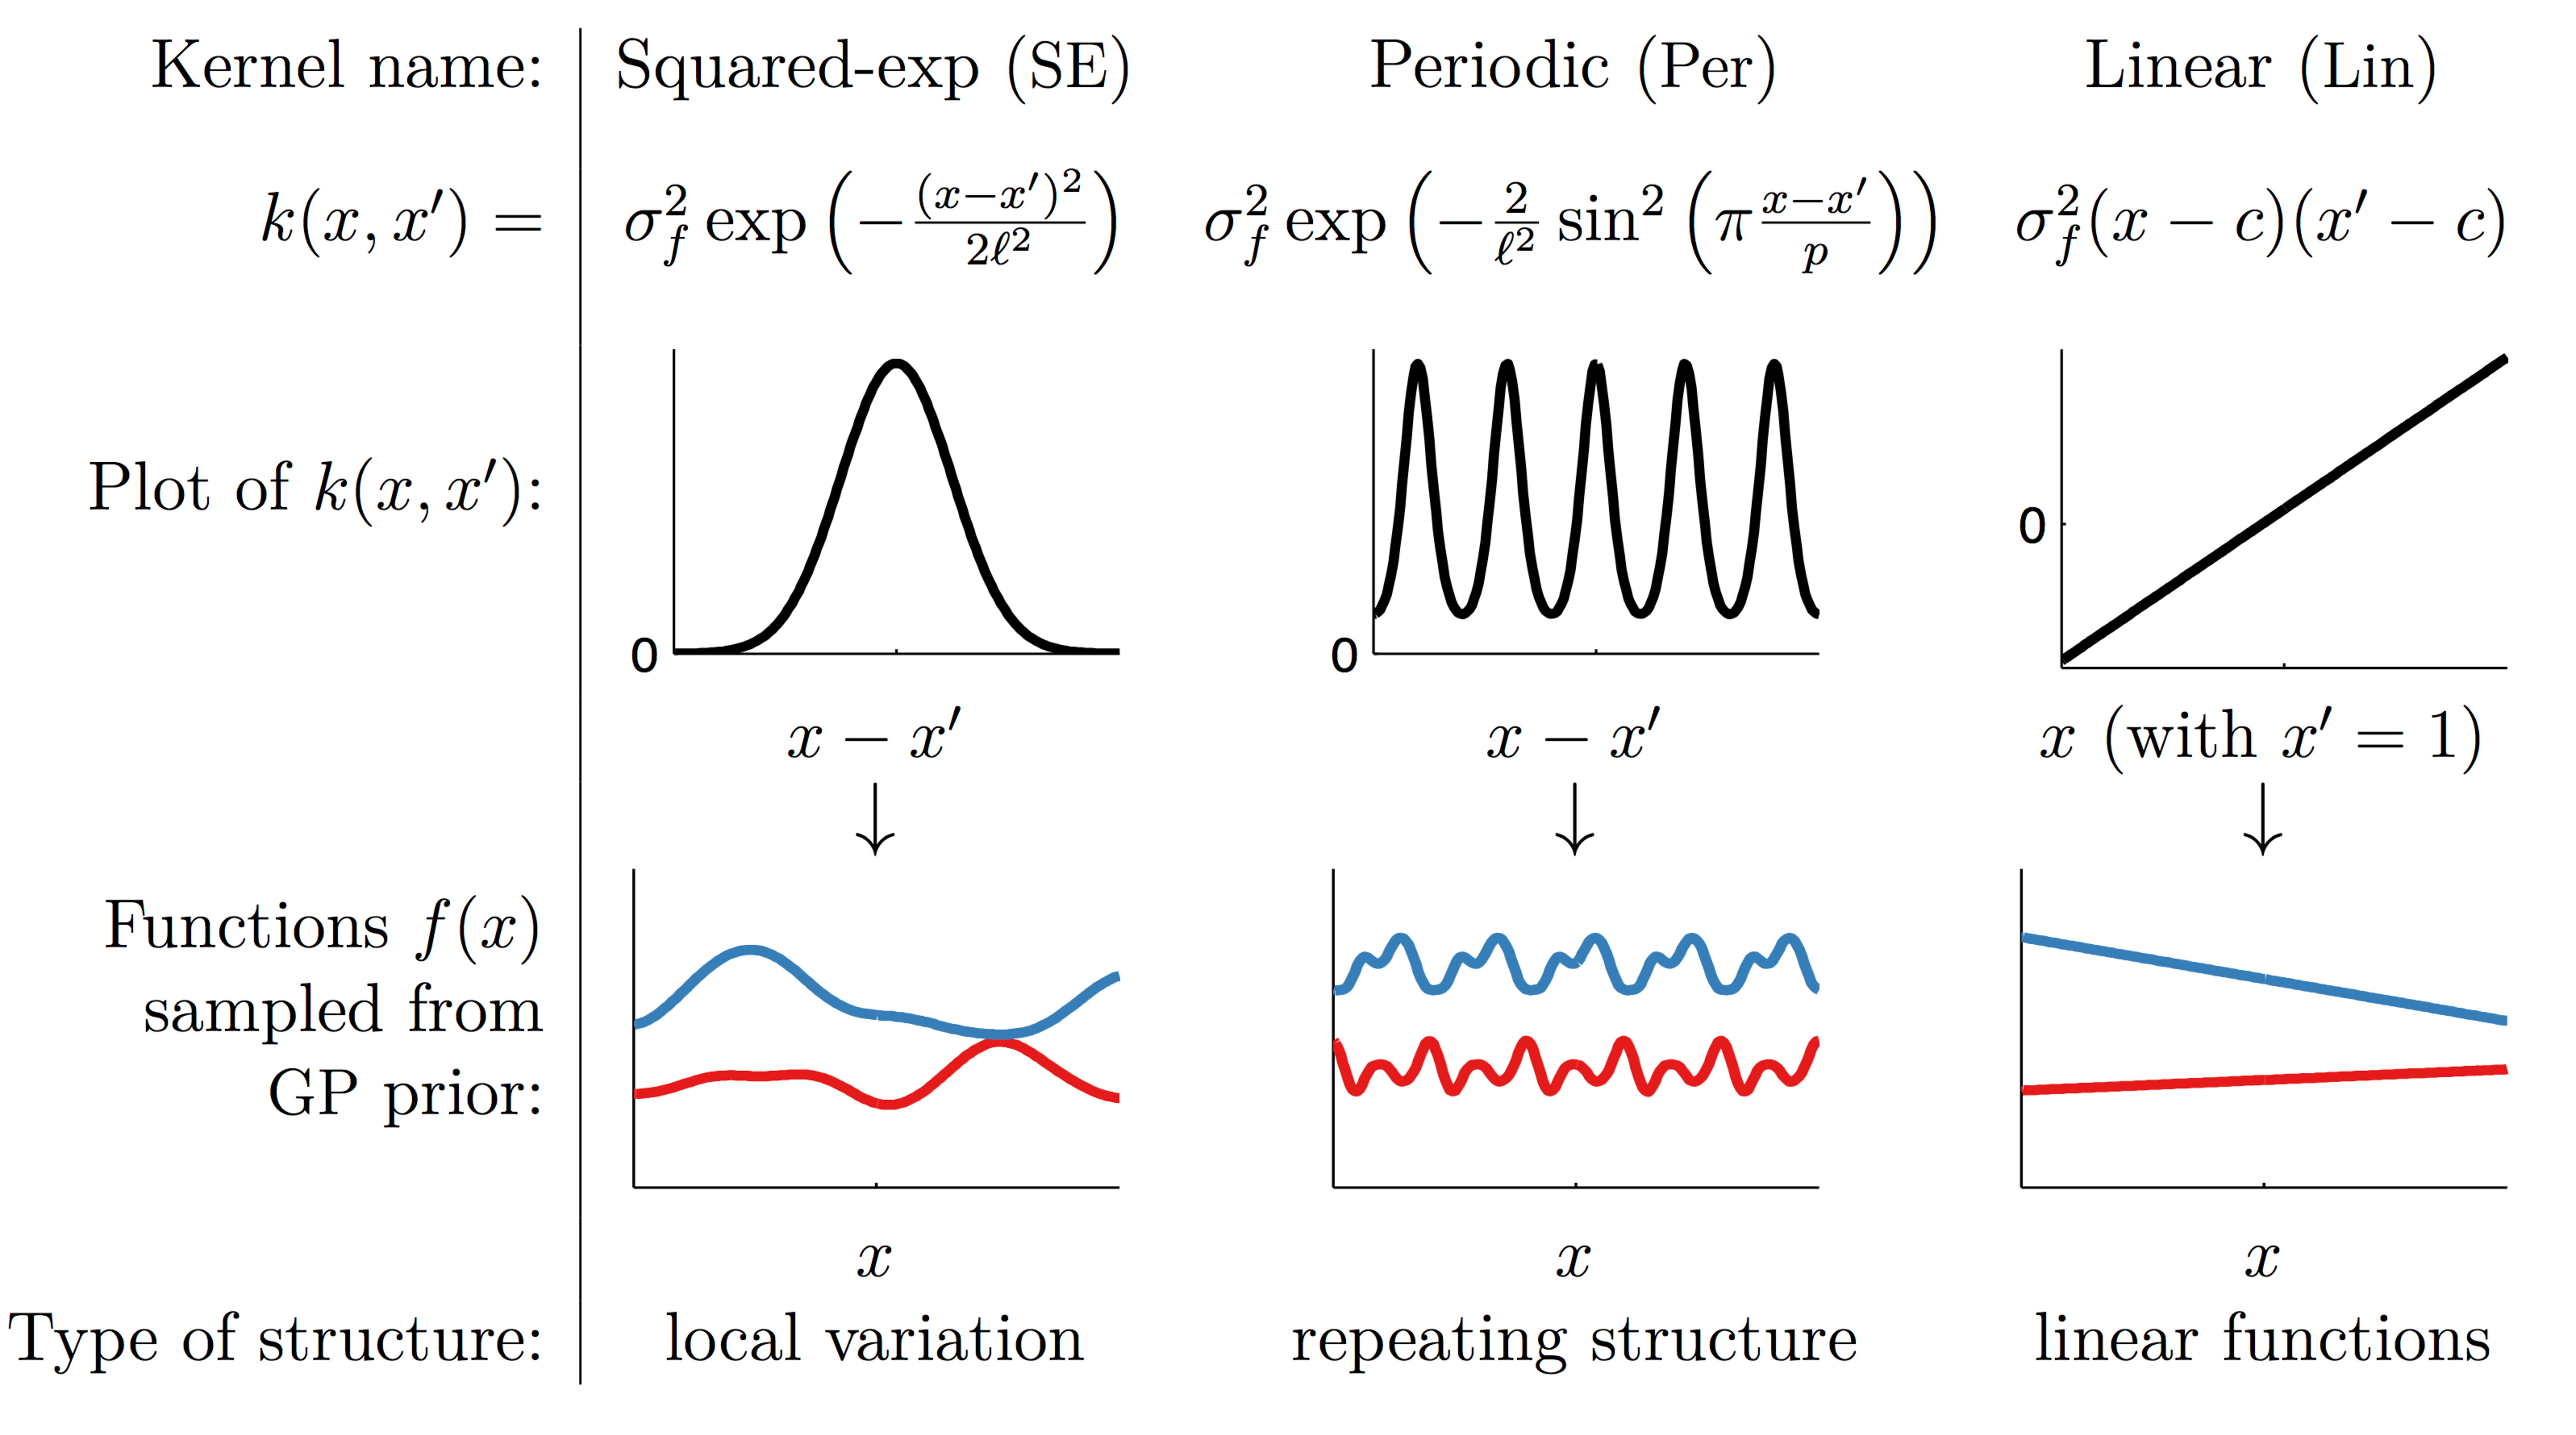
\includegraphics[width=\textwidth]{figures/kernels.pdf}
\begin{itemize}
	\item Can we specify BNN priors using GP machinery?
\end{itemize}
}

\vspace{1cm}
\mysection{Minimizing Divergence in Function Space}{

How can we find a prior on weights $p(w)$ that produces functions similar to a GP prior?

$$ \bm \phi ^* =  \amin{\bm \phi}   \E _{\X \sim p(\X)}  \kl [\pbnn (\bm f(\X) |  \bm \phi ) | \pgp (\bm f(\X )  ] $$
\begin{eqnarray*}
\kl [\pbnn (\bm f(\X) |  \bm \phi ) || \pgp (\bm f(\X )  ] = \qquad \qquad \qquad \qquad \\   
-\entropy [\pbnn (\bm f(\X) |  \bm \phi ) ]
-\E_{\pbnn (\bm f |  \bm \phi ) 
} [\log \pgp (\bm f (\X)  ) ]     
\end{eqnarray*}
We can estimate the likelihood with simple Monte Carlo, but how can we estimate the entropy of $p_{BNN}$?
%\begin{align*}
%	\E _{\X \sim p(\X)} \E_{\pbnn (\bm f |  \bm \phi ) } [\log \pgp (\bm f ( \X ) ) ]  \approx  
%  \frac{1}{S} \sum_{s=1}^S \E [\log \pgp (\bm f ^{(s)}(\X) ) ]
%\end{align*}
%where $\bm f ^{(s)}(\X) \sim \pbnn (\bm f | \X )$. What about $\entropy [\pbnn (\bm f (\X) |  \bm \phi ) ] $?
%}

}

\end{minipage}

%%% Second Column %%%%%%%%%%%%%%%%%%%%%%%%%%%%%%%%%%%%%%%%%%%%%%%%%%%%%%%%%%%%%%%
\hspace{0.25cm}
\begin{minipage}[t][47.5cm][t]{.32\textwidth}


%\vspace{1cm}
 
\mysection{Estimating the Entropy of BNN Priors}{

\col{1) Moment matching:}

Approximate {${\pbnn (\bm f (\X) |  \bm \phi ) \approx \N (\bm f | \bm \mu_{\bm f(\X) },\ \bm \Sigma _{\bm f(\X) } )}$}
using empirical mean and covariance. In this case, 
$$\entropy [\pbnn (\bm f (\X) |  \bm \phi ) ] \approx \half \log |2\pi e \bm \Sigma _{\bm f(\X) }| $$
Reasonable since $\pbnn (\bm f |  \bm \phi ) \to \pgp (\bm f  ) $ over $\X \sim p(\X)$.
\vspace{1cm}

\col{2) Nested Variational Bound:}

Introduce noise $\B y = \bm f +\bm \epsilon$, and approximate $\log p (\B y( \X)|  \bm \phi)$ with a variational lower bound $ \elbo{} (\bm \lambda, \B y^{(s)}, \bm X)$.
\begin{eqnarray*}
-\entropy [\pbnn (\B y (\X) |  \bm \phi ) ] &\approx& \frac{1}{S} \sum_{s=1}^S \log \pbnn (\B y ^{(s)}(\X)|  \bm \phi)\\ &\approx& \frac{1}{S} \sum_{s=1}^S \max_{\bm \lambda}  \elbo(\bm \lambda, \B y^{(s)}, \bm X)
\end{eqnarray*}
}
\col{3) Early stopping} to avoid mode collapse. 

\vspace{0.5cm}

\mysection{Samples from Approximate Priors}{
\setlength{\tabcolsep}{-0.25cm}

\begin{center}  
\textcolor{Green}{Gaussian Process Prior}\\
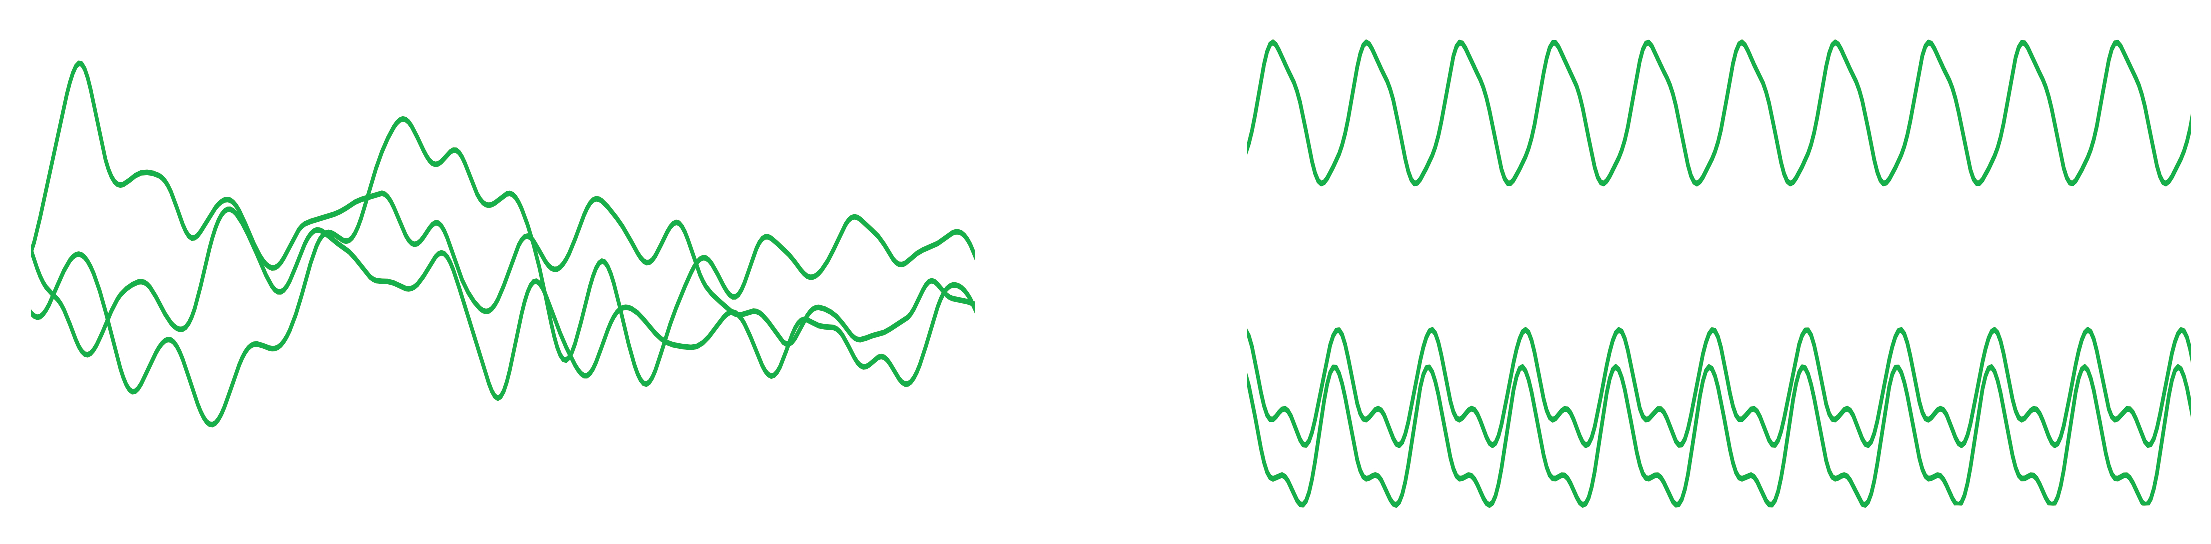
\includegraphics[width=0.8\textwidth]{figures/prior_GP.pdf}\\
%\vspace{-1cm}
%$$\textcolor{Green}{\bm f(\X) \sim \pgp (\bm f | \D )} $$
\textcolor{Blue}{Standard BNN Prior}\\
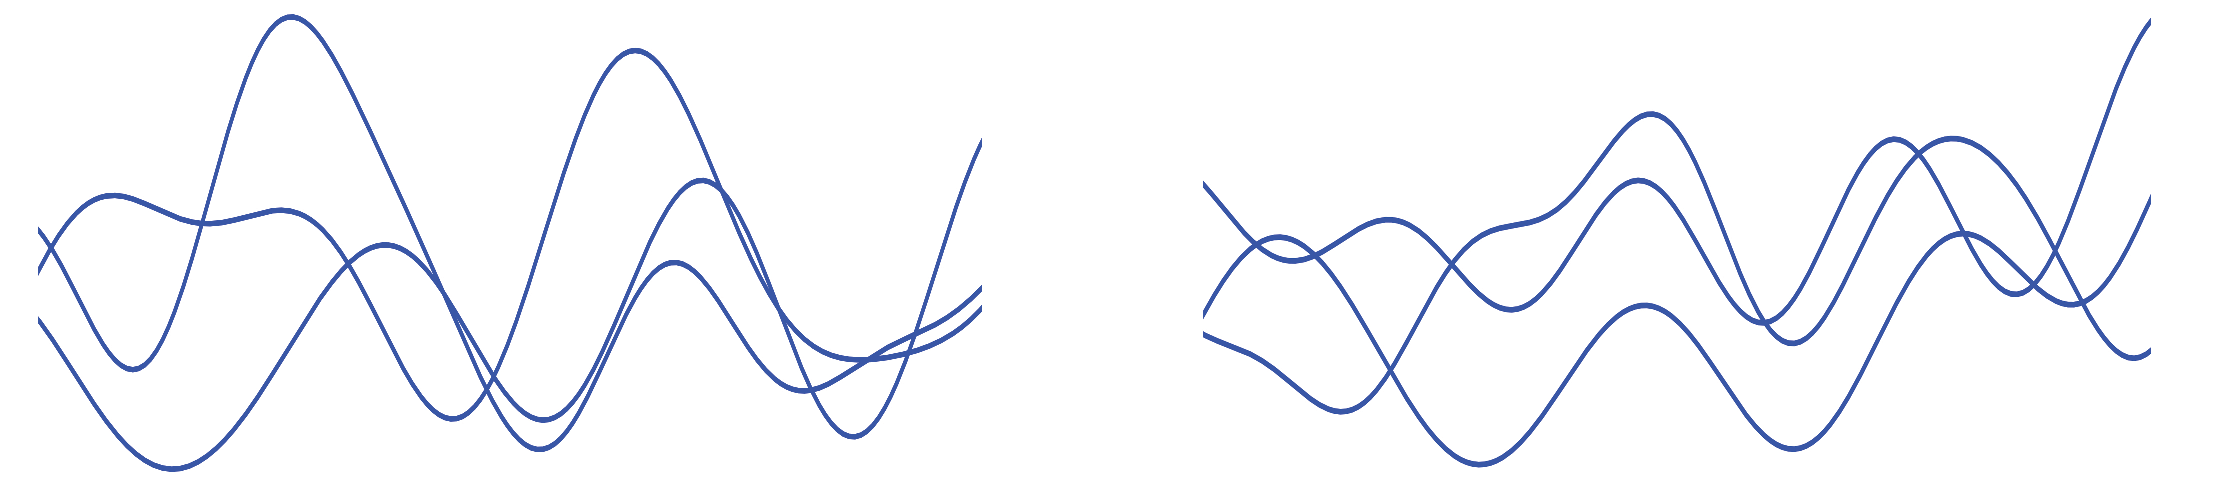
\includegraphics[width=0.8\textwidth]{figures/prior_BNN.pdf} \\   
%\vspace{-1cm}
\textcolor{Red}{GP-BNN Prior}\\
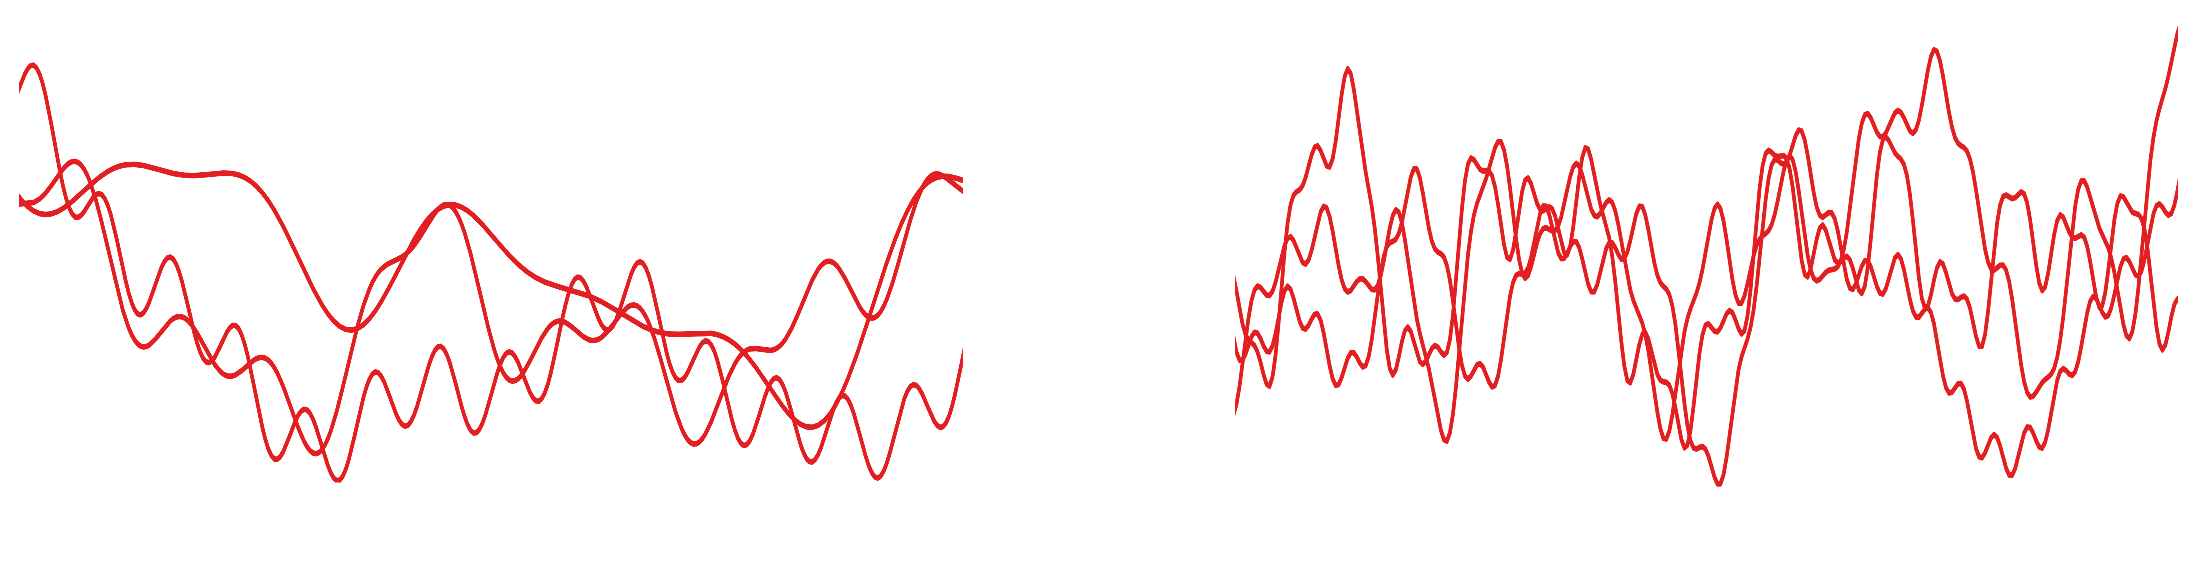
\includegraphics[width=0.8\textwidth]{figures/prior_GPBNN.pdf} \\
\end{center}


}


\end{minipage}


%%% Thirtd Column %%%
\hspace{0.5cm}
\begin{minipage}[t][14cm][t]{.3\textwidth}

%\vspace{1cm}


\mysection{Posterior Results using GP Priors}{

We test our model (blue) on 2 different toy problems. 
All BNNs are 2 layer with rbf activation functions. The GP priors used RBF kernels. 

%\hspace{2cm} $f(x) =x\sin x/10$ \hspace{4cm}  $f(x)= e^{-x^2/2} $
\begin{center}  
\textcolor{Green}{Gaussian Process Posterior}\\
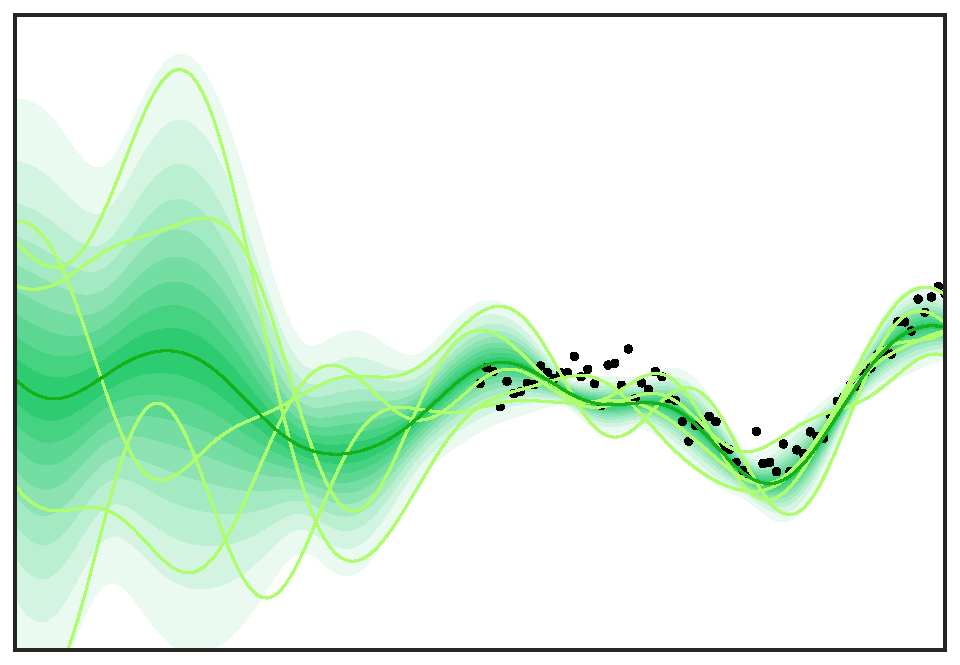
\includegraphics[width=.48\textwidth]{figures/xsinxgp.pdf}
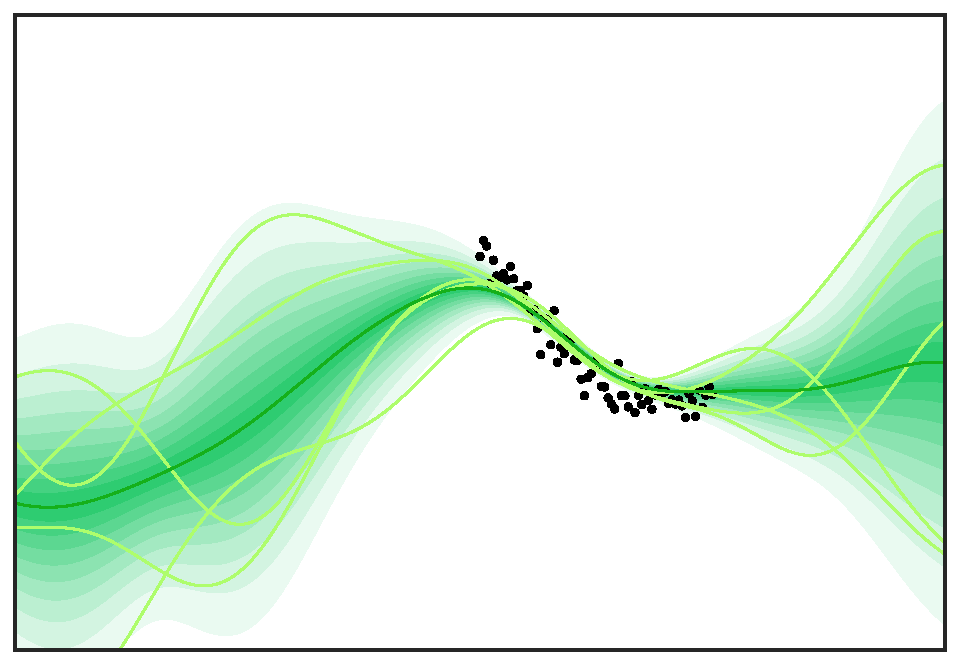
\includegraphics[width=.48\textwidth]{figures/expxgp.pdf}
%\vspace{-1cm}
%$$\textcolor{Green}{\bm f(\X) \sim \pgp (\bm f | \D )} $$
\textcolor{Blue}{Standard BNN Posterior}\\
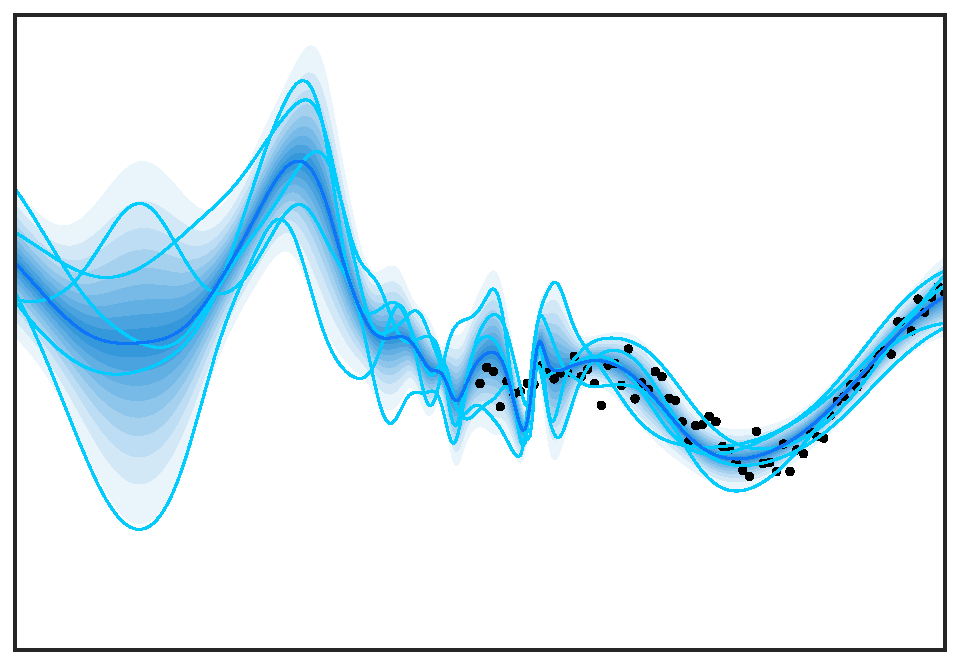
\includegraphics[width=.48\textwidth]{figures/xsinxbnn.pdf}    
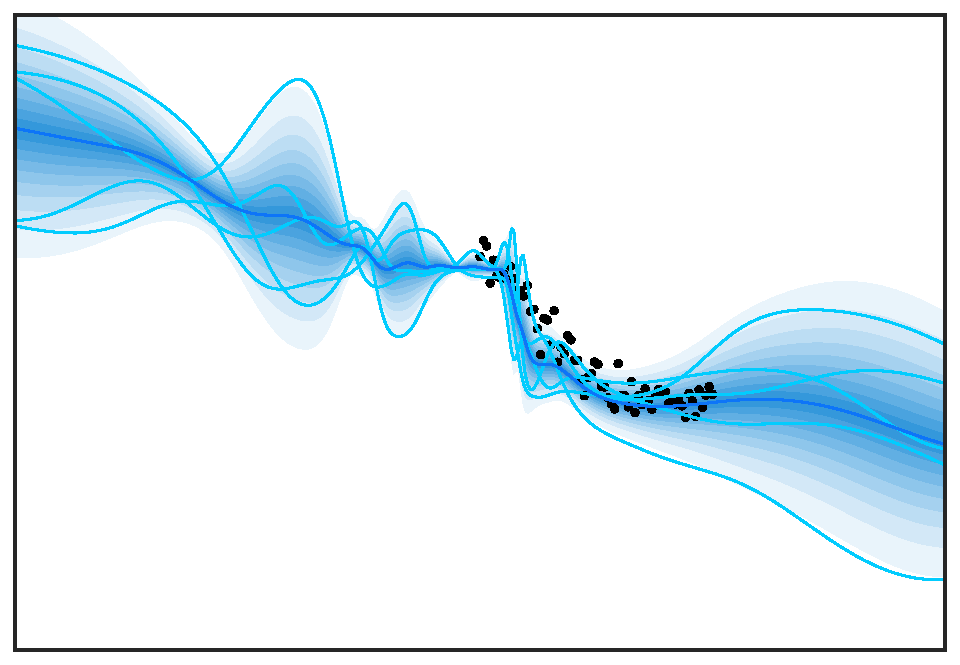
\includegraphics[width=.48\textwidth]{figures/expxbnn.pdf}       
%\vspace{-1cm}
\textcolor{Red}{GP-BNN Posterior}\\
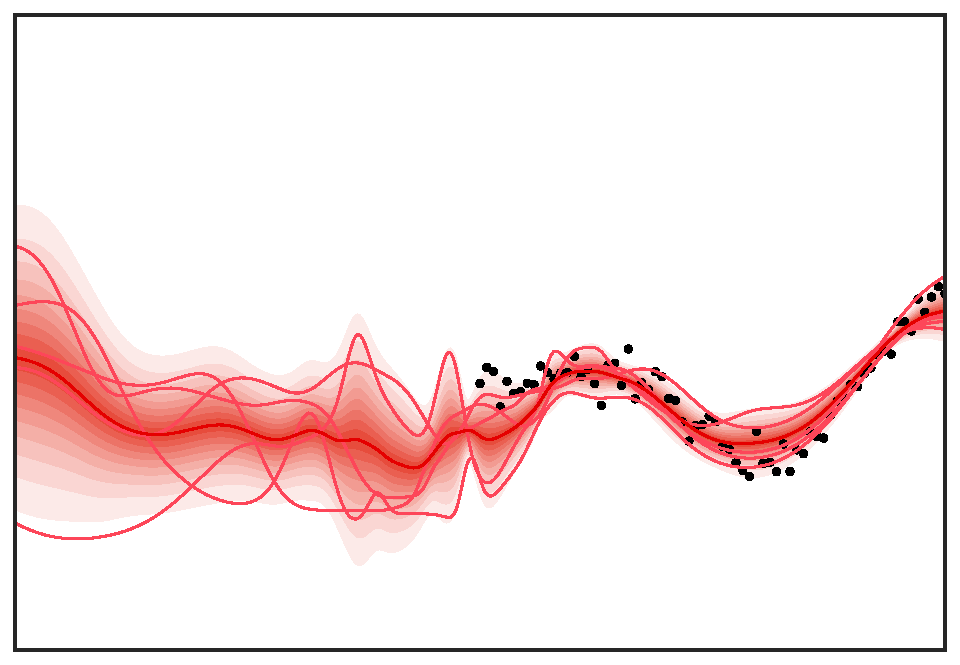
\includegraphics[width=.48\textwidth]{figures/xsinxgppbnn.pdf} 
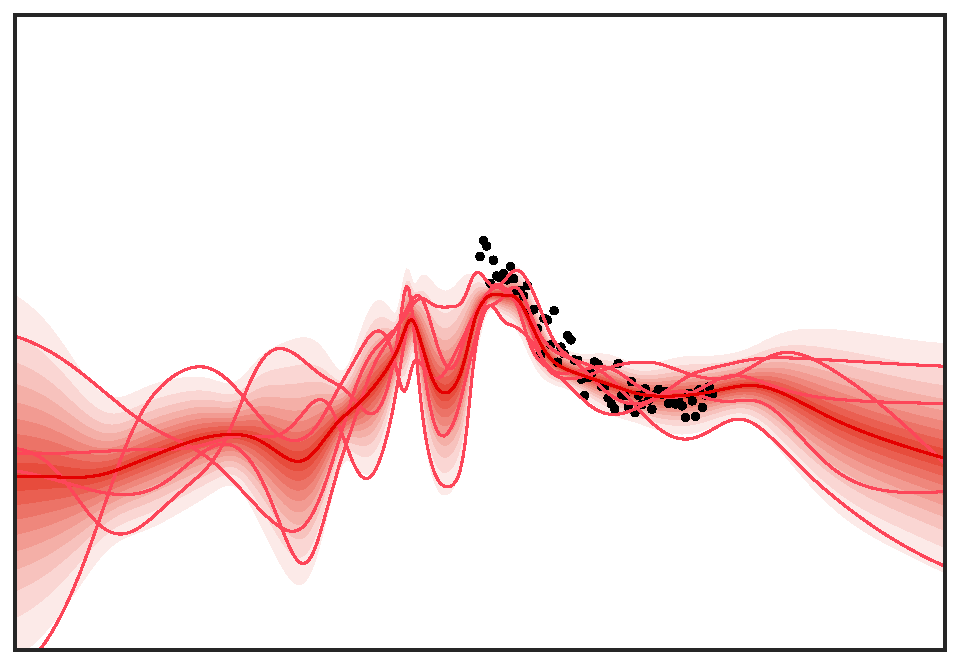
\includegraphics[width=.48\textwidth]{figures/expxgppbnn.pdf}    
%\vspace{-1cm}
%$$\textcolor{Blue}{\bm f(\X) \sim \pbnn (\bm f(\bm X)|\varphi^*) }$$
\end{center}
%\col{Results: } 
%The mean and uncertainty bands of the posterior trained with the optimized prior
%closer resembles the uncertainty of the Gaussian process. 


}

\vspace{1cm}

\mysection{Manifesto}
\begin{itemize}
\item Specifying properties of functions should be the first decision, and computational architecture follows.
\item Priors on functions are more interpretable than priors on parameters.
%\item Parameterization should be an implementation detail
\end{itemize}
\end{minipage}

\end{multicols}
\end{poster}
\end{minipage}
\end{document}

